\begin{exercise}
	Ποιος είναι ο αναγωγικός τύπος για τη μεταβλητή απόφασης $f_{mid2, i}$ στην περίπτωση σχεδιασμού έλλειψης στην περιοχή $2$ σύμφωνα με τον αλγόριθμο του Kappel;
\end{exercise}

\begin{solution}

΄Εστω ότι έχει φωτισθεί το $pixel$ $(x_{i}, y_{i})$. Επειδή βρισκόμαστε στην περιοχή 2 το επόμενο προς φωτισμό $pixel$ θα είναι το $(x_{i}-1, y_{i}+1)$ ή το $(x_{i}-1, y_{i})$ 
$$
 f_{mid2,i+1} = b^2 (x_{i}-1-1)^2 + a^2 (y_{i+1}+\frac{1}{2})^2 -a^2 b^2.
$$

Προσθαφαίροντας το $a^2(y_i + \cfrac{1}{2})^2$, προκύπτει:

\begin{align*}
    f_{mid2,i+1} &= \underbrace{b^2 (x_{i}-1)^2 + a^2 (y_{i}+\frac{1}{2})^2 -a^2 b^2}_\text{$f_{mid2,i}$} -a^2 (y_{i}+\frac{1}{2})^2 - \\
    &\qquad - 2b^2 (x_{i}-1) + b^2 + a^2 y^2_{i+1} + a^2 y_{i+1} + \frac{a^2}{4} = \\
    &= f_{mid2,i} - a^2 (y_{i}+\frac{1}{2})^2 -2b^2 (x_{i}-1) + b^2 + a^2 y^2_{i+1} + a^2 y_{i+1} + \frac{a^2}{4} = \\ 
    &= f_{mid2,i} - a^2 y^2_{i} - a^2 y_{i} - \frac{a^2}{4} -2b^2 (x_{i}-1) + b^2 + a^2 y^2_{i+1} + a^2 y_{i+1} + \frac{a^2}{4} = \\
    &= f_{mid2,i} + a^2 (y^2_{i+1} - y^2_{i}) + a^2 (y_{i+1} - y_{i}) -2b^2 (x_{i}-1) + b^2.
\end{align*}
\begin{table}[htb]
    \centering
    \begin{tabular}{@{}c|c@{}}
        \toprule
        $f_{mid2,i}$ & Επιλογή σημείου \\  \midrule
        $< 0$ & $e_i > 0 \Rightarrow$ Το $T$ πάνω από το $M$, επιλογή του σημείου $C$ \\
        $\geq 0$ & $e_i \leq 0 \Rightarrow$ Το $T$ κάτω από το $M$, επιλογή του σημείου $Β$ \\
        \bottomrule
    \end{tabular}
\end{table}
\begin{table}[htb]
    \centering
    \begin{tabular}{@{}c|c@{}} 
        \toprule
        $f_{mid2,i}<0$ &$ f_{mid2,i} -2b^2 (x_{i}-1) + b^2 + 2a^2 y_{i+1}$\\  \midrule
        $f_{mid2,i} \geq 0$ &$ f_{mid2,i} -2b^2 (x_{i}-1) + b^2 $\\
        \bottomrule  
    \end{tabular}
\end{table}
Άρα έχουμε ότι ο αναδρομικός τύπος του $f_{mid2,i}$ είναι:
\begin{gather*}
   f_{mid2,i+1} = f_{mid2,i} + a^2 (y^2_{i+1} - y^2_{i}) + a^2 (y_{i+1} - y_{i}) -2b^2 (x_{i}-1) + b^2.
\end{gather*}


\begin{figure}[hbt]
  \begin{center}
	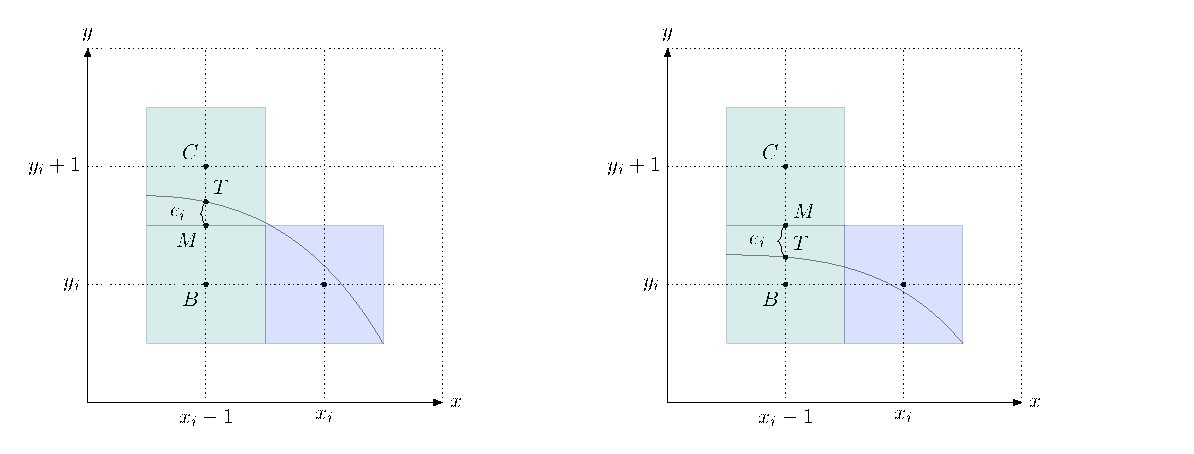
\includegraphics[scale=1]{Figures/Chapter1/Ellipse/figure4.pdf}
  \end{center}
  \caption{}
\end{figure}

	
\end{solution}
